\section{Bakgrund}

Projektet började hösten 2012 som ett internt verktyg på Developer's Helsinki efter att behov uppstått för ett system som skulle tillåta snabb implementation av anpassat innehåll på kunders webbsidor. Det bestämdes att det skulle utvecklas en mjukvara först för internt bruk men med målsättningen att lanseras som en SaaS-produkt. Mjukvaran skulle utvecklas för att vara möjligast anpassningsbar och tillåta flera olika sorters anpassningssätt. Utvecklingen genomfördes med ganska låg budget mätt både i tid och pengar, med fokus på att få ut en Minimum-Viable-Product innan företaget binder sig till den.

\subsection{Developer's Helsinki}

Developer's Helsinki Oy är ett finskt företag som utvecklar såväl applikationstjänster (jfr. engelskans \gls{saas}) som webbsidor. Företaget grundades 2009 för att vidareutveckla  \gls{saas}-tjänsten Netmonitor, en produktfamilj bestående av webbanalys och marknadsföringsverktyg.

Företaget har en stark kännedom av marknadsföring på webben efter att ha jobbat med både utvecklingen av webbsidor samt uppföljningen av resultat genom webbanalys. På basis av denna erfarenhet började SmartElement-projektet planeras. Kunskapen fanns inom företaget och genom att anpassa processer från webbanalys sågs en möjlighet för automatisering av anpassning av innehåll.

\subsection{Anpassat innehåll}

\begin{figure}[h!]
\centering
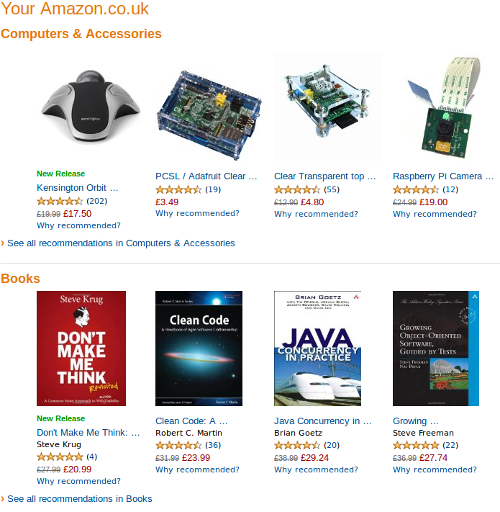
\includegraphics[width=120mm]{assets/images/amazon.png}
\caption{Amazons användarsida med anpassat innehåll}
\label{amazon}
\end{figure}

Anpassat innehåll, eller personaliserat innehåll (eng. \textit{Personalized content}), är innehåll som väljs ut på basis av egenskaper hos användaren. I fallet av webbsidor kan det handla om information så som användarens geografiska läge, användarens språk, användarens webbläsare, antalet besök som användaren gjort till sidan m.m. Tanken är att förse användaren med det den behöver, eller vill ha, utan att denne behöver be om det. \citep{cotacm43}

Anpassat innehåll har bland annat använts inom nätbutiker för att visa reklam anpassad för kunden på basis av dennes beställningshistorik. Figur \ref{amazon} visar användarsidan som visas då man loggar in på Amazons webb-butik. Inom social media används anpassat innehåll för att lyfta fram innehåll som antas vara intressant för användaren, så som t.ex. uppdateringar från vänner som användaren ofta är i kontakt med eller reklam från företag användaren har gillat. \citep{socialmedia}

Anpassning av innehåll kan anses ha börjat med de första webbsidorna som tillåtit inloggning och på så vis anpassat webbsidan för en återvändande användare. Man kan anse att så lite som en användarinformationsbox för inloggade användare är anpassning av innehåll. I dagens läge menar man oftast mera avancerad anpassning baserad på segmentering av användare och klassificering av innehåll.

En för de flesta bekant form av anpassning av webbinnehåll är anpassade sökresultat. Söktjänsten Google har sedan 2004 använt sig av anpassade sökresultat. Sedan 2009 anpassas sökresultat dessutom för icke autentiserade besökare \citep{Hannak:2013:MPW:2488388.2488435}. Googles anpassade sökresultat kan ses som en föregångare för anpassat webbinnehåll, de har presenterat konceptet för en bred publik.

Anpassningen av innehåll kan åstadkommas på olika sätt. Ofta handlar det om användning av statistik för att välja ut innehåll som motsvarar en besökares uppvisade intressen. Det kan handla om en så enkel sak som att använda statistiken för att visa en liten hälsning för återkommande besökare. Det finns dock mera avancerade metoder för anpassning, så som att använda information som besökaren förser webbsidan med i kombination med användarens beteende på sidan för att klassificera denne. \citep{Albanese:2004:WPB:1031453.1031469} 

\subsection{Behov}

I takt med att stora aktörer införde allt mer anpassat innehåll så började även mindre aktörers kunder fråga om möjligheten att använda tekniken på sina webbsidor. Det visade sig att det inte fanns något företag på finska marknaden som erbjöd ett tillräckligt flexibelt system för anpassning av innehåll och därmed bestämdes det att Developer's Helsinki skulle utveckla ett sådant.

Systemet skulle kunna leverera innehåll dels i form av text (HTML eller rå text) för direkt injicering i webbsidans \gls{dom}, dels i form av data i \gls{json} format och dels som \gls{jsonp} svar, vilket tillåter exekvering av JavaScript vid svaret. För filtrering skulle det samlas in data om besökares webbläsare och dator, men det skulle även vara möjligt att tillägga egen data som sedan kunde användas för filtrering.

\section{Befintliga lösningar}

I takt med att anpassning av webbinnehåll blivit mer populärt har det utvecklats olika lösningar för ändamålet. Det finns i dagens läge såväl kommersiella produkter som open-sourceprojekt som erbjuder olika typer av anpassningssystem. På open-sourcefronten handlar det oftast om webbinnehållsplattformer som innehåller en anpassningsmodul som en del av helheten. På den kommersiella sidan finns det många lösningar för optimering av webbutiker genom anpassning av innehållet på sidan.

\subsection{Kommersiella lösningar}

Vid tillfället för beslutet att utveckla produkten var den enda kommersiella lösningen på finska marknaden nosto.com som levererar anpassat innehåll med inriktning på webbutiker. Systemet är utformat att förse upprätthållare av webbutiker med verktyg för optimering av konversioner samt för att uppehålla kundrelationer. \citep{nosto}

Nosto har valt en tydlig kundgrupp, systemet utvecklas för att passa in i webbutikers verksamhet. SmartElement utformades, till skillnad från Nosto, som ett generellt system för anpassning av innehåll på webbsidor av alla typer. Nosto är en större helhet, som inte bara innefattar anpassat innehåll.

Den kommersiella lösning som närmast liknar SmartElement i funktionalitet är Personyze. Systemet bygger på en liknande lösning som SmartElement var upprätthållaren av en webbsida skapar regler för vilka besökarsegment som skall se specifik information och lägger till i sin sida en kort JavaScript-kod, vilken sedan hämtar innehåll som passar användaren. \citep{personyze}

\subsection{Lösningar baserade på öppen källkod}

På open-sourcefronten finns det bl.a. webbinnehållsplattformen Pimcore som innehåller en anpassningsmotor. Funktionaliteten baserar sig på att skapa besökarsegment. Efter konfiguration kan upprätthållaren, medan denne editerar en sida, välja ett besökarsegment att anpassa innehållet för \citep{pimcore}.
Till skillnad från SmartElement är Pimcore en hel plattform för hantering av webbinnehåll. För att använda plattformen måste upprätthållaren ta i bruk systemet samt upprätthålla en server var systemet kan köras. SmartElement är däremot tänkt som en tjänst för upprätthållare att lägga till på sin befintliga sida, oberoende av underliggande system.

Ett mera tekniskt krävande system för utveckling av anpassat innehåll är PredictionIO. Det är ett maskininlärningssystem baserat på öppen källkod som kan användas för att automatiskt generera anpassade rekommendationer för besökare. Systemet bygger på att man skapar en motor som sedan tränas genom att mata in beteendedata om användare i relation till olika ting. \citep{predicionioconcepts}


% vim: set tw=78:ts=2:sw=2:et:fdm=marker:wrap:wm=78:ft=tex
% vim: spell spelllang=sv
